This is a 1-D problem that consists of a domain with 3 regions of differing
saturation values $\frac{q}{\sigma}$. This is used to test both reaction
terms and source terms.
Table \ref{tab:three_region} summarizes the test parameters.

%-------------------------------------------------------------------------------
\begin{table}[htb]\caption{Three-Region Test Problem Summary}
\label{tab:three_region}
\centering
\begin{tabular}{l l}\toprule
\emph{Parameter} & \emph{Value}\\\midrule
Domain & $\mathcal{D} = (0,1)$\\
Initial Conditions & $u_0(\x)=0$\\
Boundary Conditions & $u(\x,t)=u_{inc}=1,\quad \x\in\partial\mathcal{D}^-,\quad t>0,$\\
   & $\partial\mathcal{D}^-=\{\x\in\partial\mathcal{D}:\mathbf{n}(\x)
     \cdot\mathbf{\Omega}<0\}$\\
Direction & $\mathbf{\Omega} = \mathbf{e}_x$\\
Cross Section & $\sigma(\x)=\left\{\begin{array}{c l}
   \sigma_0, & x\in[x_0,x_1]\\
   \sigma_1, & x\in(x_1,x_2]\\
   \sigma_2, & x\in(x_2,x_3]
   \end{array}\right.,\quad
   \left[\begin{array}{c}\sigma_0\\\sigma_1\\\sigma_2\end{array}\right] =
      \left[\begin{array}{c}1\\40\\20\end{array}\right]$\\
   & $\left[\begin{array}{c}x_0\\x_1\\x_2\\x_3\end{array}\right] =
      \left[\begin{array}{c}0\\0.3\\0.6\\1\end{array}\right]$\\
Source & $q(\x,t)=\left\{\begin{array}{c l}
   q_0, & x\in[x_0,x_1]\\
   q_1, & x\in(x_1,x_2]\\
   q_2, & x\in(x_2,x_3]
   \end{array}\right.,\quad
   \left[\begin{array}{c}q_0\\q_1\\q_2\end{array}\right] =
      \left[\begin{array}{c}1\\5\\20\end{array}\right]$\\
Speed & $c=1$\\
Exact Solution & $u(\x,t) = u_b + u_q$\\
   & $u_b=\tilde{u_0}(x-ct)e^{-\tau},
        \quad N_r=3,\quad
        \tau = \sum\limits_{i=0}^{N_r-1} \sigma_i s_i,$\\
   & $\tilde{u_0}(x) = \left\{\begin{array}{l l}
        u_{inc}, & x<x_0\\
        0,       & x\geq 0
     \end{array}\right.$,\\
   & $u_q=\sum\limits_{i=0}^{N_r-1}u_{q,i}e^{-\tau_i},\quad
        \tau_i = \sum\limits_{j=i+1}^{N_r-1} \sigma_j s_j,$\\
   & $u_{q,i} = \left\{\begin{array}{l l}
        \frac{q_i}{\sigma_i}\left(1-e^{-\sigma_i s_i}\right), & \sigma_i\neq 0\\
        q_i s_i, & \sigma_i = 0
        \end{array}\right.$,\\
   & $s_i = \max(s^+_i-s^-_i,0)$,\\
   & $s^+_i = \min(x,x_{i+1}),\quad
     s^-_i = \max(x-ct,x_i)$ \\
\bottomrule\end{tabular}
\end{table}
%-------------------------------------------------------------------------------

Figure \ref{fig:three_region} compares the solutions computed
for each scheme for this problem, and
Table \ref{tab:three_region_run_parameters} shows the run parameters used.
%-------------------------------------------------------------------------------
\begin{table}[ht]\caption{Three-Region Test Problem Run Parameters}
\label{tab:three_region_run_parameters}
\centering
\begin{tabular}{l l}\toprule
\emph{Parameter} & \emph{Value}\\\midrule
Number of Cells & $N_{cell} = 2^5 = 32$\\
End Time & $t = 1$\\
CFL Number & $\nu = 0.5$\\
Time Integrator & SSPRK33\\\midrule
Entropy Function & $E(u) = \frac{1}{2}u^2$\\
Entropy Residual Coefficient & $c_E = 0.1$\\
Entropy Jump Coefficient & $c_J = 0.1$\\
Entropy Time Integrator & BE\\
\bottomrule\end{tabular}
\end{table}
%-------------------------------------------------------------------------------
\begin{figure}[ht]
   \centering
   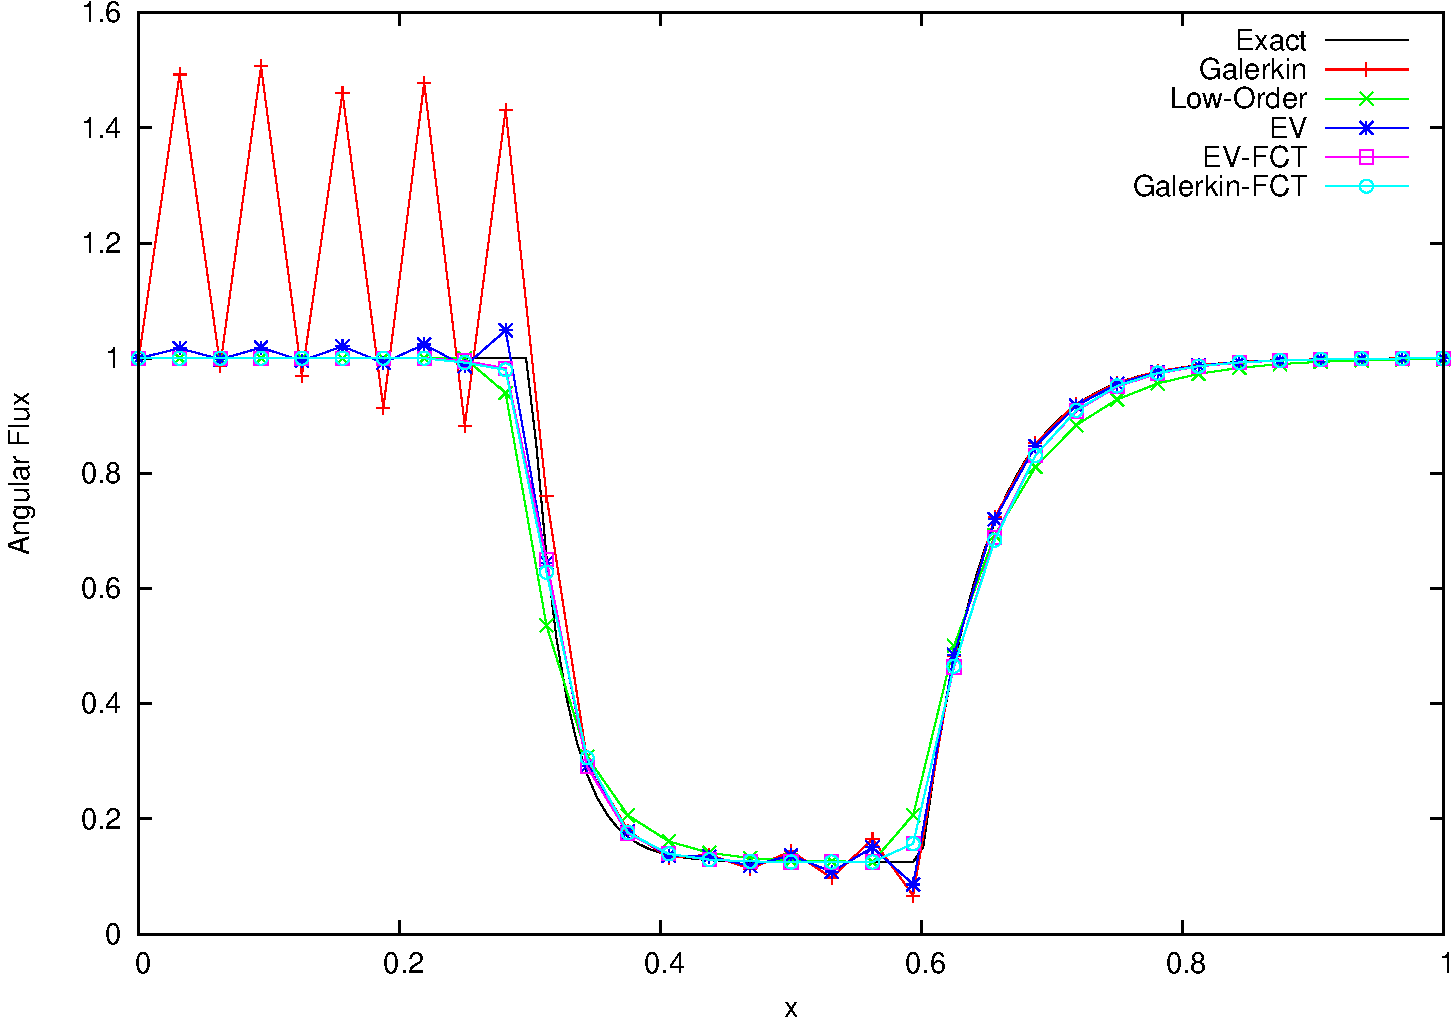
\includegraphics[width=0.9\textwidth]
     {\contentdir/results/transport/three_region/three_region.pdf}
   \caption{Comparison of Solutions for the 3-Region Test Problem}
   \label{fig:three_region}
\end{figure}
%-------------------------------------------------------------------------------

\clearpage
